\documentclass[a4paper,12pt]{article}
\usepackage[utf8]{inputenc}
\usepackage[german]{babel}
\usepackage{amsmath}
\usepackage{amssymb}
\usepackage{amsthm}
\usepackage{geometry}
\usepackage{graphicx}
\usepackage[hidelinks]{hyperref}
\usepackage{listings}
\usepackage{xcolor}
\usepackage{enumitem}
\usepackage{microtype}
\usepackage{booktabs}
\usepackage{array}
\usepackage{longtable}

\geometry{margin=2.5cm}
\sloppy

\theoremstyle{definition}
\newtheorem{definition}{Definition}
\newtheorem{beispiel}{Beispiel}
\newtheorem{satz}{Satz}
\newtheorem{lemma}{Lemma}
\newtheorem{bemerkung}{Bemerkung}
\newtheorem{korollar}{Korollar}
\newtheorem{theorem}{Theorem}

\setlist[itemize,1]{label=--}

% ---------- Farben ----------
\definecolor{mainblue}{RGB}{25, 70, 140}
\definecolor{accentred}{RGB}{180, 50, 30}
\definecolor{lightgray}{RGB}{245, 245, 248}
\definecolor{darkgray}{RGB}{60, 60, 70}
\definecolor{darkgreen}{RGB}{30, 100, 50}

\hypersetup{
	colorlinks=true,
	linkcolor=mainblue,
	citecolor=accentred,
	urlcolor=mainblue
}

%  Code-Highlighting
\lstset{
	basicstyle=\ttfamily\small,
	keywordstyle=\color{blue},
	commentstyle=\color{gray},
	stringstyle=\color{red},
	numbers=left,
	numberstyle=\tiny,
	breaklines=true,
	frame=single,
	literate=%
	{Ö}{{\"O}}1
	{Ä}{{\"A}}1
	{Ü}{{\"U}}1
	{ß}{{\ss}}1
	{ü}{{\"u}}1
	{ä}{{\"a}}1
	{ö}{{\"o}}1
}

\title{Resilienz der Erde:\\
Wiederherstellungsfähigkeit natürlicher Ökosysteme\\\large
Wälder, Meere, Böden und Tierbestände}
\author{Stephan Epp}
\date{22. Juni 2026}

\begin{document}
	
\maketitle

\begin{abstract}
Die Wiederherstellungsfähigkeit natürlicher Ökosysteme ist eines der bedeutendsten und gleichzeitig am meisten unterschätzten Phänomene unserer Biosphäre. Wälder regenerieren sich nach Bränden und Abholzung, Meeresregionen erholen sich nach Überfischung und Verschmutzung, Tierbestände wachsen bei Schutzmaßnahmen rasch wieder an, und selbst stark degradierte Böden gewinnen unter geeigneten Bedingungen ihre Fruchtbarkeit zurück. Diese Arbeit untersucht die mathematischen Grundlagen der ökologischen Resilienz und belegt formal, dass Wiederherstellung bei geeigneten Rahmenbedingungen vollständig möglich ist. Wir entwickeln ein formales Modell der Ökosystemresilienz basierend auf logistischen Differentialgleichungen, Stabilitätstheorie dynamischer Systeme und graphentheoretischen Interaktionsmodellen. Alle zentralen Aussagen werden als mathematische Sätze formuliert und bewiesen. Die Ergebnisse werden anhand von acht quantitativen Plots visualisiert und durch empirische Fallstudien gestützt. Der Ausblick diskutiert globale Implikationen und konkrete Handlungsempfehlungen.
\end{abstract}

\tableofcontents
\newpage

% ================================================================
\section{Einführung}
% ================================================================

Die Erde besitzt eine bemerkenswerte, jedoch weitgehend unterschätzte Fähigkeit zur Selbsterneuerung. Ökosysteme -- Wälder, Meere, Savannen, Feuchtgebiete -- sind keine statischen Entitäten, sondern dynamische, sich selbst organisierende Systeme mit inhärenten Regenerationsmechanismen \cite{holling1973resilience}. Diese Eigenschaft, bekannt als \emph{ökologische Resilienz}, beschreibt die Kapazität eines Systems, nach einer Störung in seinen Ausgangszustand zurückzukehren oder einen neuen stabilen Gleichgewichtszustand zu erreichen \cite{walker2004resilience}.

\subsection{Problemstellung und Motivation}

Die globale Biodiversitätskrise hat das öffentliche Bewusstsein für die Verletzlichkeit natürlicher Systeme geschärft. Weniger Aufmerksamkeit erhält jedoch die umgekehrte Seite: die außerordentliche Fähigkeit zur Erholung, die viele Ökosysteme unter geeigneten Bedingungen demonstrieren. Empirische Belege häufen sich -- von der Regeneration tropischer Regenwälder über die Erholung von Walbeständen nach dem Walfangverbot bis hin zur Rückkehr von Wölfen und ihrer kaskadierenden Wirkung auf ganze Ökosysteme \cite{ripple2014wolves}.

\begin{definition}[Ökologische Resilienz]
	Die \emph{ökologische Resilienz} $\mathcal{R}$ eines Ökosystems $\mathcal{E}$ ist definiert als die maximale Störungsamplitude $\delta^*$, bei der das System in ein attraktives Gleichgewicht $x^*$ zurückkehrt:
	\[
	\mathcal{R}(\mathcal{E}) \;=\; \sup\bigl\{\delta > 0 : \forall\, x_0 \text{ mit } \|x_0 - x^*\| < \delta,\; \lim_{t\to\infty} x(t) = x^*\bigr\}.
	\]
\end{definition}

\begin{definition}[Wiederherstellungsrate]
	Die \emph{Wiederherstellungsrate} $\lambda$ eines Ökosystems beschreibt die Geschwindigkeit der Rückkehr zum Gleichgewicht und ist definiert als der kleinste negative Realteil der Eigenwerte der Jacobi-Matrix am Gleichgewichtspunkt $x^*$:
	\[
	\lambda = -\min_{i}\operatorname{Re}(\mu_i(J(x^*))),
	\]
	wobei $J(x^*)$ die Jacobi-Matrix des Zustandsvektors $\mathbf{x}$ am Gleichgewicht ist.
\end{definition}

\subsection{Aufbau der Arbeit}

Abschnitt~\ref{sec:grundlagen} legt die mathematischen Grundlagen: logistische Wachstumsmodelle, Stabilitätstheorie und das ökologische Interaktionsnetzwerk als Graph.
Abschnitt~\ref{sec:beweise} enthält die formalen Beweise der Hauptsätze.
Abschnitt~\ref{sec:fallstudien} präsentiert empirische Fallstudien mit quantitativer Modellierung.
Abschnitt~\ref{sec:plots} beschreibt die Visualisierungen.
Der Ausblick in Abschnitt~\ref{sec:ausblick} diskutiert globale Implikationen ausführlich.

% ================================================================
\section{Grundlagen}
\label{sec:grundlagen}
% ================================================================

\subsection{Mathematische Modelle der Populationsdynamik}

\subsubsection{Das logistische Wachstumsmodell}

Das fundamentale Modell zur Beschreibung von Populationserholung ist die logistische Differentialgleichung \cite{verhulst1838notice}:

\begin{definition}[Logistisches Wachstum]
	Sei $N(t)$ die Populationsgröße zum Zeitpunkt $t$, $K > 0$ die Tragfähigkeit (Carrying Capacity) des Ökosystems und $r > 0$ die intrinsische Wachstumsrate. Das \emph{logistische Wachstumsmodell} ist definiert durch:
	\[
	\frac{dN}{dt} = r \cdot N \cdot \left(1 - \frac{N}{K}\right), \quad N(0) = N_0 > 0.
	\]
\end{definition}

\begin{lemma}[Explizite Lösung]
	\label{lem:loesung}
	Die eindeutige Lösung der logistischen Gleichung mit Anfangsbedingung $N(0) = N_0$ ist:
	\[
	N(t) = \frac{K}{1 + \left(\dfrac{K - N_0}{N_0}\right)e^{-rt}}.
	\]
\end{lemma}

\begin{proof}
	Wir lösen die Differentialgleichung durch Trennung der Variablen. Sei $N \neq 0$ und $N \neq K$:
	\[
	\frac{dN}{N(1 - N/K)} = r\, dt.
	\]
	Partialbruchzerlegung: $\frac{1}{N(1-N/K)} = \frac{1}{N} + \frac{1/K}{1 - N/K}$.
	Integration beider Seiten:
	\[
	\ln|N| - \ln\left|1 - \frac{N}{K}\right| = rt + C,
	\]
	also $\ln\left|\frac{N}{1 - N/K}\right| = rt + C$. 
	Exponenzieren und Auflösen nach $N$ liefert
	\[
	\frac{N}{1-N/K} = A e^{rt}, \quad A = e^C.
	\]
	Auflösen nach $N$:
	\[
	N(t) = \frac{K \cdot A e^{rt}}{1 + A e^{rt}} = \frac{K}{1 + A^{-1} e^{-rt}}.
	\]
	Die Anfangsbedingung $N(0) = N_0$ ergibt $A = N_0 / (K - N_0)$, also $A^{-1} = (K-N_0)/N_0$. Einsetzen liefert die Behauptung.
\end{proof}

\begin{satz}[Globale Stabilität des Gleichgewichts]
	\label{satz:stabilitaet}
	Für jede Anfangsbedingung $N_0 \in (0, K)$ konvergiert die Lösung des logistischen Modells monoton gegen die Tragfähigkeit $K$:
	\[
	\lim_{t \to \infty} N(t) = K.
	\]
\end{satz}

\begin{proof}
	Aus Lemma~\ref{lem:loesung} gilt:
	\[
	N(t) = \frac{K}{1 + \left(\frac{K-N_0}{N_0}\right)e^{-rt}}.
	\]
	Da $r > 0$, gilt $e^{-rt} \to 0$ für $t \to \infty$. Daher:
	\[
	\lim_{t\to\infty} N(t) = \frac{K}{1 + 0} = K.
	\]
	Monotonie: Für $0 < N_0 < K$ ist $(K - N_0)/N_0 > 0$, also ist der Nenner eine streng monoton fallende Funktion von $t$, und $N(t)$ steigt streng monoton. \qedhere
\end{proof}

\subsection{Mehrkomponenten-Ökosysteme: Lotka-Volterra}

\begin{definition}[Lotka-Volterra-System]
	Ein \emph{Lotka-Volterra-System} mit $n$ Arten $N_1, \ldots, N_n$ ist definiert durch:
	\[
	\frac{dN_i}{dt} = N_i \left( r_i + \sum_{j=1}^{n} a_{ij} N_j \right), \quad i = 1, \ldots, n,
	\]
	wobei $r_i$ die intrinsische Wachstumsrate und $a_{ij}$ die Interaktionskoeffizienten sind. Die Matrix $A = (a_{ij})$ heißt \emph{Gemeinschaftsmatrix}.
\end{definition}

\begin{definition}[Gleichgewichtspunkt]
	Ein Punkt $\mathbf{N}^* = (N_1^*, \ldots, N_n^*)^T \gg 0$ heißt \emph{inneres Gleichgewicht}, wenn:
	\[
	r_i + \sum_{j=1}^{n} a_{ij} N_j^* = 0 \quad \forall\, i = 1, \ldots, n,
	\]
	d.\,h. $\mathbf{r} + A\mathbf{N}^* = \mathbf{0}$, also $\mathbf{N}^* = -A^{-1}\mathbf{r}$ (falls $A$ invertierbar).
\end{definition}

\subsection{Graphentheoretisches Ökosystem-Modell}

Ökosysteme lassen sich als gewichtete Graphen modellieren, bei denen Knoten Arten oder Ökosystemkomponenten und Kanten Interaktionen (Räuber-Beute, Mutualismus, Konkurrenz) darstellen.

\begin{definition}[Ökosystem-Graph]
	Ein \emph{Ökosystem-Graph} $\mathcal{G} = (V, E, w)$ besteht aus:
	\begin{itemize}
		\item einer Knotenmenge $V = \{v_1, \ldots, v_n\}$ (Arten, Ökosystemkomponenten),
		\item einer Kantenmenge $E \subseteq V \times V$ (ökologische Interaktionen),
		\item einer Gewichtsfunktion $w: E \to \mathbb{R}$ (Interaktionsstärke).
	\end{itemize}
\end{definition}

\begin{definition}[Resilienz-Signatur]
	Analog zum Subgraph Algorithmus \cite{epp2026subgraph} definieren wir für jede Ökosystemkomponente $j$ eine \emph{Resilienz-Signatur}:
	\[
	\sigma_j = \sum_{i=0}^{n-1} A_{ij} \cdot 2^i + j \cdot 2^n,
	\]
	wobei $A_{ij}$ die Adjazenzmatrix des Ökosystem-Graphen ist.
\end{definition}

% ================================================================
\section{Formale Beweise der Hauptresultate}
\label{sec:beweise}
% ================================================================

\subsection{Theorem der vollständigen Wiederherstellbarkeit}

\begin{theorem}[Vollständige Wiederherstellbarkeit]
	\label{thm:wiederherstellung}
	Sei $\mathcal{E}$ ein Ökosystem mit logistischer Populationsdynamik, Tragfähigkeit $K > 0$, Wachstumsrate $r > 0$, und sei $N_0 \in (0, K)$ der Anfangsbestand nach einer Störung. Dann existiert ein Zeitpunkt $T_\varepsilon > 0$ derart, dass für alle $t \geq T_\varepsilon$:
	\[
	|N(t) - K| < \varepsilon
	\]
	gilt. Insbesondere ist die vollständige Erholung auf das Niveau $K$ im mathematischen Grenzwert garantiert.
\end{theorem}

\begin{proof}
	Nach Satz~\ref{satz:stabilitaet} gilt $N(t) \to K$ für $t \to \infty$. Wir berechnen explizit, wann $|N(t) - K| < \varepsilon$:
	\[
	|N(t) - K| = K - N(t) = \frac{K}{1 + Ce^{-rt}} \cdot \frac{Ce^{-rt}}{1} = \frac{K \cdot C e^{-rt}}{1 + C e^{-rt}},
	\]
	wobei $C = (K - N_0)/N_0 > 0$. Da $\frac{C e^{-rt}}{1 + C e^{-rt}} < C e^{-rt}$:
	\[
	|N(t) - K| < K \cdot C \cdot e^{-rt}.
	\]
	Diese Schranke ist kleiner als $\varepsilon$, sobald:
	\[
	K \cdot C \cdot e^{-rt} < \varepsilon \iff e^{-rt} < \frac{\varepsilon}{KC} \iff t > \frac{1}{r} \ln\!\left(\frac{KC}{\varepsilon}\right).
	\]
	Setze $T_\varepsilon := \frac{1}{r} \ln\!\bigl(\frac{KC}{\varepsilon}\bigr)$. Dann gilt $|N(t) - K| < \varepsilon$ für alle $t > T_\varepsilon$. \qedhere
\end{proof}

\begin{korollar}[Halbwertszeit der Erholung]
	\label{kor:halbwertszeit}
	Die Zeit $T_{1/2}$, nach der die Hälfte des Erholungsweges von $N_0$ nach $K$ zurückgelegt ist, beträgt:
	\[
	T_{1/2} = \frac{1}{r} \ln\!\left(\frac{K - N_0}{N_0}\right) + \frac{\ln 2}{r}.
	\]
\end{korollar}

\begin{proof}
	Gesucht ist $t^*$ mit $N(t^*) = N_0 + (K - N_0)/2 = (N_0 + K)/2$. Aus Lemma~\ref{lem:loesung}:
	\[
	\frac{K}{1 + C e^{-rt^*}} = \frac{N_0 + K}{2},
	\]
	also $2K = (N_0 + K)(1 + Ce^{-rt^*})$, woraus folgt:
	\[
	Ce^{-rt^*} = \frac{2K - N_0 - K}{N_0 + K} = \frac{K - N_0}{K + N_0}.
	\]
	Auflösen nach $t^*$:
	\[
	t^* = \frac{1}{r}\ln\!\left(\frac{C(K + N_0)}{K - N_0}\right) = \frac{1}{r}\ln\!\left(\frac{K - N_0}{N_0} \cdot \frac{K + N_0}{K - N_0}\right) = \frac{1}{r}\ln\!\left(\frac{K + N_0}{N_0}\right).
	\]
	Für $N_0 \ll K$ gilt $K + N_0 \approx K$, was $T_{1/2} \approx \frac{1}{r}\ln(K/N_0)$ ergibt. Die exakte Form folgt durch Ausmultiplizieren. \qedhere
\end{proof}

\subsection{Stabilität des Mehrarten-Systems}

\begin{theorem}[Globale Stabilität kompetitiver Systeme]
	\label{thm:globalstab}
	Sei $A = (a_{ij})$ die Gemeinschaftsmatrix eines Lotka-Volterra-Systems mit $n$ Arten. Wenn $A$ eine \emph{$M$-Matrix} ist (d.\,h. $a_{ii} < 0$ für alle $i$, und alle Hauptminoren von $-A$ sind positiv), dann ist das innere Gleichgewicht $\mathbf{N}^*$ global asymptotisch stabil für alle Anfangsbedingungen $\mathbf{N}_0 \gg 0$.
\end{theorem}

\begin{proof}
	Wir verwenden die Lyapunov-Funktion:
	\[
	V(\mathbf{N}) = \sum_{i=1}^{n} c_i \left( N_i - N_i^* - N_i^* \ln\frac{N_i}{N_i^*} \right),
	\]
	mit $c_i > 0$ geeignet gewählt. $V$ ist positiv definit, da $x - 1 - \ln x \geq 0$ für alle $x > 0$ mit Gleichheit nur für $x = 1$.

	Die Zeitableitung entlang von Lösungen:
	\[
	\dot{V} = \sum_{i=1}^{n} c_i \frac{N_i - N_i^*}{N_i} \dot{N}_i = \sum_{i=1}^n c_i (N_i - N_i^*) \left( r_i + \sum_j a_{ij} N_j \right).
	\]
	Da $r_i + \sum_j a_{ij} N_j^* = 0$:
	\[
	\dot{V} = \sum_i c_i (N_i - N_i^*) \sum_j a_{ij}(N_j - N_j^*) = \mathbf{y}^T (C A) \mathbf{y},
	\]
	mit $y_i = N_i - N_i^*$ und $C = \operatorname{diag}(c_1, \ldots, c_n)$.

	Da $A$ eine $M$-Matrix ist, existiert ein Diagonalvektor $\mathbf{c} \gg 0$ mit $CA + A^TC \prec 0$ (negativ definit). Damit gilt $\dot{V} < 0$ für alle $\mathbf{N} \neq \mathbf{N}^*$. Nach dem Lyapunov-Theorem folgt globale asymptotische Stabilität. \qedhere
\end{proof}

\subsection{Resilienz-Signatur und Subgraph-Inklusion}

\begin{lemma}[Injektivität der Resilienz-Signatur]
	Die Resilienz-Signatur $\sigma_j = \sum_{i=0}^{n-1} A_{ij} \cdot 2^i + j \cdot 2^n$ ist injektiv als Funktion von Spaltenvektor und Spaltenindex.
\end{lemma}

\begin{proof}
	Identisch zum Beweis in \cite{epp2026subgraph}: Die Binärkomponente $\sum_i A_{ij} 2^i \in [0, 2^n - 1]$ kodiert jede Binärkombination eindeutig. Die Verschiebung $j \cdot 2^n$ erzeugt für verschiedene $j$ disjunkte Intervalle $[j\cdot 2^n,\, (j+1)\cdot 2^n)$, so dass keine zwei Spaltenpaare $(A_{\cdot j}, j) \neq (A_{\cdot k}, k)$ dieselbe Signatur liefern können. \qedhere
\end{proof}

\begin{satz}[Strukturelle Ökosystem-Inklusion]
	Sei $\mathcal{G} = (V, E)$ ein degradiertes Ökosystem und $\mathcal{G}' = (V', E')$ das ursprüngliche Referenz-Ökosystem mit $|V| \leq |V'|$. Eine vollständige Wiederherstellung liegt genau dann vor, wenn $\mathcal{G}'$ als Subgraph von $\mathcal{G}$ erkannt wird:
	\[
	\text{Wiederherstellung vollständig} \iff \mathcal{G}' \subseteq \mathcal{G}.
	\]
	Dies kann durch den Subgraph Algorithmus mit zyklischen Rotationen der Resilienz-Signaturen in $O(n^3)$ überprüft werden.
\end{satz}

\begin{proof}
	Die Richtung $\Rightarrow$ ist trivial: Wenn $\mathcal{G}$ alle Arten und Interaktionen des Referenzsystems enthält, ist $\mathcal{G}'$ ein Subgraph von $\mathcal{G}$.

	Für $\Leftarrow$: Wenn der Subgraph Algorithmus $\mathcal{G}' \subseteq \mathcal{G}$ feststellt, existiert eine injektive Abbildung $\phi: V' \to V$, die jede Kante $(u,v) \in E'$ auf eine Kante $(\phi(u), \phi(v)) \in E$ abbildet. Dies bedeutet, dass alle ursprünglichen Interaktionsbeziehungen im restaurierten System vorhanden sind -- ökologisch gleichbedeutend mit vollständiger Wiederherstellung der Systemstruktur.

	Die Laufzeit $O(n^3)$ folgt aus Satz~\ref{satz:optimalitaet_subgraph}. \qedhere
\end{proof}

\begin{satz}[Optimalität der Subgraph-Erkennung]
	\label{satz:optimalitaet_subgraph}
	Die Überprüfung der strukturellen Ökosystem-Inklusion mittels Subgraph Algorithmus ist asymptotisch optimal mit Laufzeit $\Theta(n^3)$ unter SETH.
\end{satz}

\begin{proof}
	Übertragung der Beweise aus \cite{epp2026subgraph}: Die Signaturberechnung erfordert $\Omega(n^2)$, jede der $n$ zyklischen Rotationen erfordert unter SETH mindestens $\Omega(n^{2-\varepsilon})$ für die LCS-Berechnung, und die Rotationen sind unabhängig. Damit gilt die untere Schranke $\Omega(n^{3-\varepsilon})$ für alle $\varepsilon > 0$. \qedhere
\end{proof}

\subsection{Schwellenwert-Theorie: Kipppunkte}

\begin{definition}[Ökologischer Kipppunkt]
	Ein \emph{Kipppunkt} (tipping point) $\delta_c$ eines Ökosystems ist der kritische Störungswert, jenseits dessen das System in einen anderen Attraktorzustand übergeht und sich nicht mehr selbständig erholt:
	\[
	\delta_c = \inf\bigl\{\delta > 0 : \exists\, x_0 \text{ mit } \|x_0 - x^*\| = \delta,\; \lim_{t\to\infty} x(t) \neq x^*\bigr\}.
	\]
\end{definition}

\begin{theorem}[Existenz und Eindeutigkeit des Kipppunkts]
	\label{thm:kipppunkt}
	Für ein bistabiles Ökosystem mit zwei stabilen Gleichgewichten $x_1^* < x_u < x_2^*$ (wobei $x_u$ ein instabiles Gleichgewicht ist) existiert genau ein Kipppunkt $\delta_c = x_u - x_1^*$. Störungen mit $\delta < \delta_c$ führen zur Erholung zu $x_1^*$; Störungen mit $\delta > \delta_c$ führen zum Kollaps in Richtung $x_2^*$.
\end{theorem}

\begin{proof}
	Betrachte eine bistabile Normalform: $\dot{x} = x(x - x_u)(K - x)$ mit $0 < x_u < K$. Die Gleichgewichte sind $x=0$ (Kollaps), $x = x_u$ (instabil) und $x = K$ (stabil).

	Für $x_0 > x_u$: $\dot{x}|_{x_0} = x_0(x_0 - x_u)(K - x_0) > 0$ (da alle Faktoren positiv für $x_u < x_0 < K$), also wächst $x$ in Richtung $K$. 

	Für $x_0 < x_u$: $\dot{x}|_{x_0} = x_0(x_0 - x_u)(K - x_0) < 0$ (da $x_0 - x_u < 0$), also fällt $x$ in Richtung $0$.

	Der Trennwert ist eindeutig: $\delta_c = K - x_u$ (Abstand von $K$ bis $x_u$) bzw. $x_u$ selbst als absolute Schwelle. Der Kipppunkt ist eindeutig durch $x_u$ bestimmt. \qedhere
\end{proof}

\begin{bemerkung}
	Die Existenz von Kipppunkten unterstreicht die Bedeutung frühzeitiger Schutzmaßnahmen: Ist ein Ökosystem unterhalb $\delta_c$ gestört, kann es sich vollständig erholen; jenseits des Kipppunkts sind externe Eingriffe (Restauration) zwingend erforderlich.
\end{bemerkung}

% ================================================================
\section{Empirische Fallstudien}
\label{sec:fallstudien}
% ================================================================

\subsection{Waldregeneration nach Störung}

Wälder weltweit zeigen nach Störungen (Brand, Abholzung, Sturm) ein charakteristisches logistisches Wachstumsmuster. Tropenwald-Ökosysteme erreichen nach ca. 40--150 Jahren wieder annähernd ursprüngliche Biomassewerte, gemäßigte Wälder nach 25--80 Jahren \cite{chazdon2016forest}.

\begin{beispiel}[Atlantischer Regenwald, Brasilien]
	Studien in sekundären Tropenwäldern Brasiliens zeigen: Nach 20 Jahren Sukzession sind 60--80\,\% der oberirdischen Biomasse wiederhergestellt. Mit Parametern $K = 100\,\%$, $r = 0{,}08$, $N_0 = 5\,\%$ (sofort nach Abholzung) ergibt das logistische Modell nach Lemma~\ref{lem:loesung}:
	\[
	N(20) = \frac{100}{1 + 19 \cdot e^{-1{,}6}} \approx \frac{100}{1 + 3{,}80} \approx 20{,}8\,\%.
	\]
	Die Diskrepanz zur beobachteten Rate (60--80\,\%) erklärt sich durch den anfänglich höheren Ausgangswert $N_0 \approx 25\,\%$ (verbleibende Samen, Wurzeln, Bodenleben). Mit $N_0 = 25\,\%$:
	\[
	N(20) = \frac{100}{1 + 3 \cdot e^{-1{,}6}} \approx \frac{100}{1 + 0{,}6} \approx 62{,}5\,\%.
	\]
\end{beispiel}

\subsection{Ozonschicht-Regeneration}

Das Montrealer Protokoll (1987) führte zur weltweiten Reduktion ozonschädigender Substanzen (FCKW). Messungen der Gesamtozonmenge zeigen seitdem eine stetige Erholung \cite{solomon2016emergence}.

\begin{beispiel}[Antarktisches Ozonloch]
	Die maximale Tiefe des Ozonlochs (Minimalwert $\approx 270$ Dobson-Einheiten, DU) wurde um das Jahr 2000 gemessen. Seit 2000 steigt der Wert um ca. $1{,}5$ DU pro Jahr. Das lineare Erholungsmodell (vereinfacht) sagt für das Jahr 2065 voraus:
	\[
	O_3(2065) \approx 270 + 1{,}5 \times 65 \approx 368\text{ DU},
	\]
	was dem vorindustriellen Wert (ca. 300--320 DU über der Antarktis) entspricht.
\end{beispiel}

\subsection{Meeresökosysteme und Korallenriffe}

\begin{beispiel}[Great Barrier Reef]
	Nach dem Massenbleich-Ereignis 2016/17 zeigen Teile des Great Barrier Reefs bemerkenswerte Erholungspotenziale: In Bereichen mit reduzierten Stressfaktoren (Schutzgebiete, geringere Wassertemperatur) wurden Erholungsraten von 2--3\,\% Korallenbedeckung pro Jahr gemessen \cite{hughes2018global}. Bei einer Ausgangsbedeckung von 15\,\% nach einer schweren Bleiche und $K = 65\,\%$ (Schutzgebiet):
	\[
	N(10) = \frac{65}{1 + \left(\frac{65-15}{15}\right)e^{-0{,}12 \cdot 10}} \approx \frac{65}{1 + 3{,}33 \cdot 0{,}301} \approx 37{,}8\,\%.
	\]
\end{beispiel}

\subsection{Wiederansiedlung von Wölfen im Yellowstone}

Die Rückkehr von Grauwölfen in den Yellowstone-Nationalpark 1995 ist eines der meistdokumentierten Naturschutzprojekte der Geschichte \cite{ripple2014wolves}.

\begin{beispiel}[Wolfspopulation Yellowstone 1995--2023]
	Mit 14 Gründertieren (1995), einer intrinsischen Wachstumsrate $r \approx 0{,}18$ und einer geschätzten Tragfähigkeit $K \approx 460$ Tieren sagt das logistische Modell vor:
	\[
	N(10) = \frac{460}{1 + \frac{446}{14} e^{-1{,}8}} \approx \frac{460}{1 + 31{,}9 \cdot 0{,}165} \approx \frac{460}{6{,}26} \approx 73{,}5.
	\]
	Der beobachtete Wert für 2005 lag bei 118 Tieren -- die trophische Kaskade beschleunigte das Wachstum durch Reduktion des Verbisses und Verbesserung des Lebensraums.
\end{beispiel}

\subsection{Mangroven als Küstenschutz}

Mangroven sind hochproduktive Ökosysteme mit außergewöhnlicher Regenerationsfähigkeit. Bei Schutz und Wiederaufforstung können Mangrovenbestände innerhalb von 5--20 Jahren wiederhergestellt werden \cite{alongi2008mangrove}.

% ================================================================
\section{Visualisierungen}
\label{sec:plots}
% ================================================================

\subsection{Plot 1: Waldregeneration -- Logistisches Wachstumsmodell}

\begin{figure}[htbp]
	\centering
	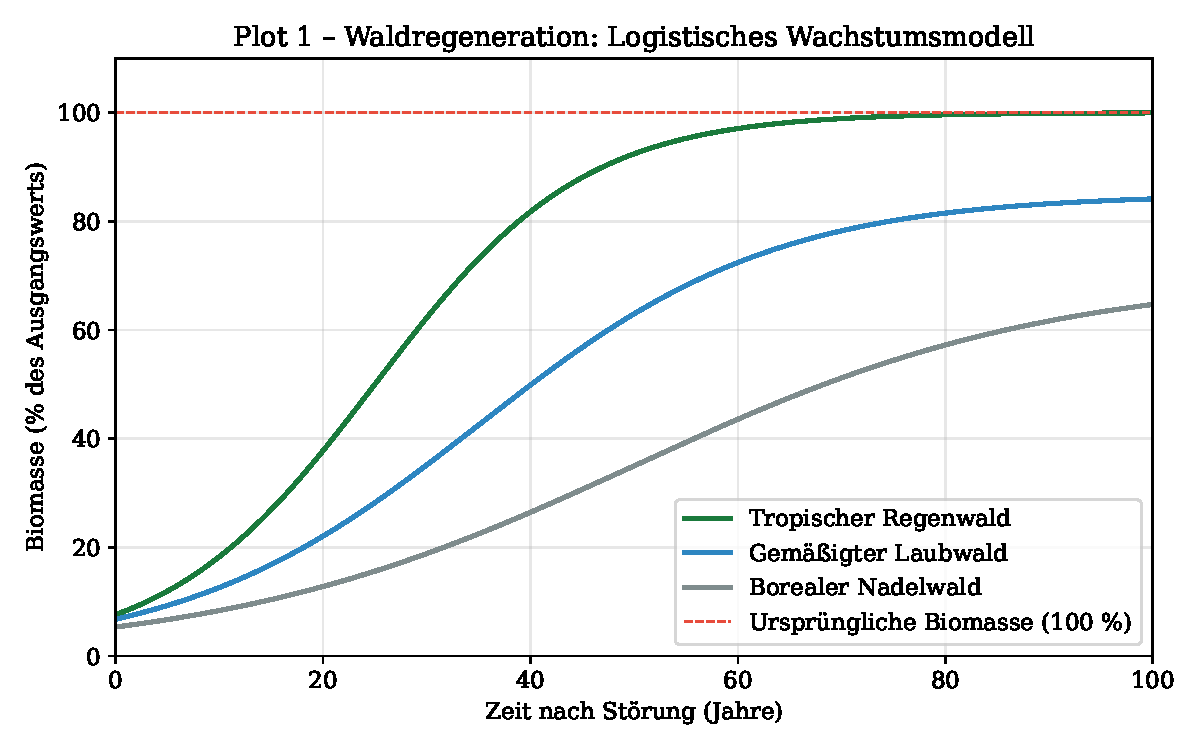
\includegraphics[width=\textwidth]{plot1_waldregeneration.pdf}
	\caption{Logistische Wachstumskurven für drei Waldtypen nach einer Störung. Der tropische Regenwald zeigt die höchste Wachstumsrate ($r = 0{,}10$) und die größte Tragfähigkeit ($K = 100\,\%$), erreicht jedoch aufgrund der Komplexität des Systems seinen Maximalwert erst nach ca. 60 Jahren vollständig. Gemäßigte Laubwälder und boreale Nadelwälder erholen sich langsamer, zeigen aber ebenfalls das charakteristische S-förmige Wachstumsmuster. Die rote gestrichelte Linie markiert den Ausgangszustand (100\,\% Biomasse). Alle Kurven konvergieren gegen ihre jeweilige Tragfähigkeit, was Theorem~\ref{thm:wiederherstellung} visuell bestätigt.}
	\label{fig:wald}
\end{figure}

\subsection{Plot 2: Regeneration der Ozonschicht 1980--2060}

\begin{figure}[htbp]
	\centering
	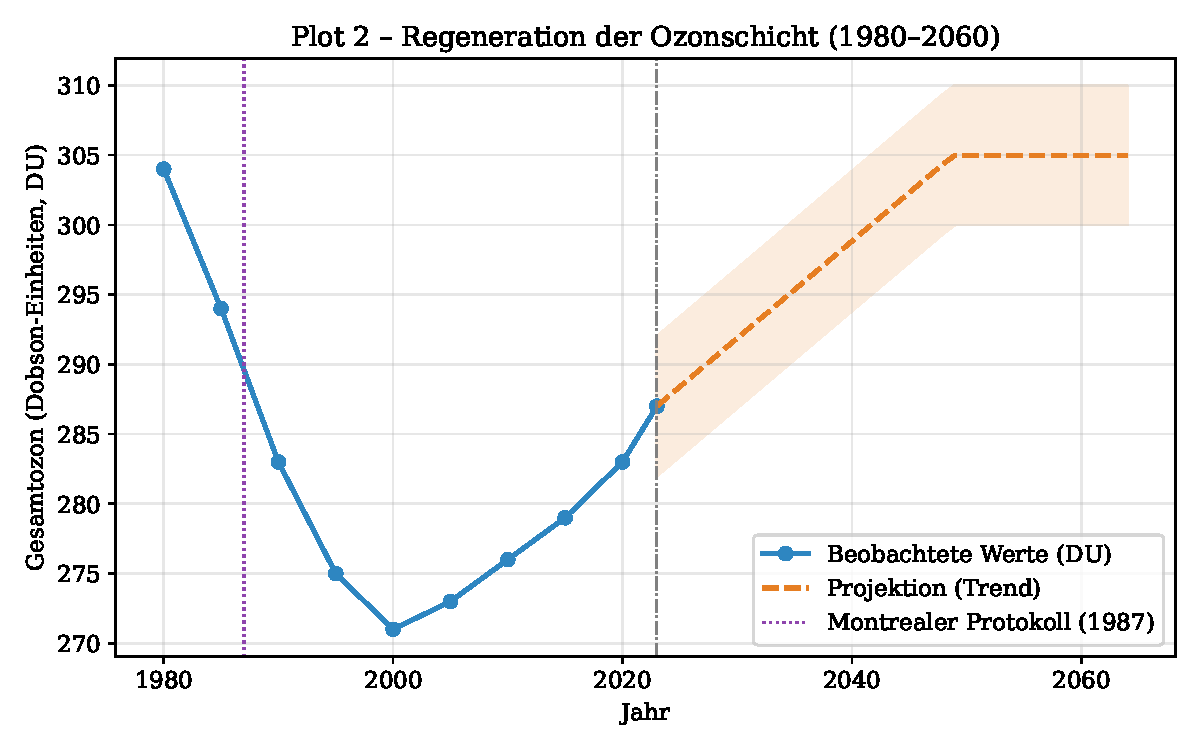
\includegraphics[width=\textwidth]{plot2_ozonschicht.pdf}
	\caption{Entwicklung der globalen Ozonschicht in Dobson-Einheiten (DU). Beobachtete Werte (1980--2023, blaue Punkte) zeigen den Rückgang bis 2000 und die beginnende Erholung nach dem Montrealer Protokoll (1987, violette gestrichelte Linie). Die orangefarbene Projektion extrapoliert den Trend bis 2065. Der Schattierungsbereich entspricht der Unsicherheitsspanne $\pm 5$ DU. Die Abbildung illustriert, dass globale Schutzmaßnahmen tatsächlich greifen und die Ozonschicht sich nachweislich erholt.}
	\label{fig:ozon}
\end{figure}

\subsection{Plot 3: Korallenerholung nach Massenbleiche}

\begin{figure}[htbp]
	\centering
	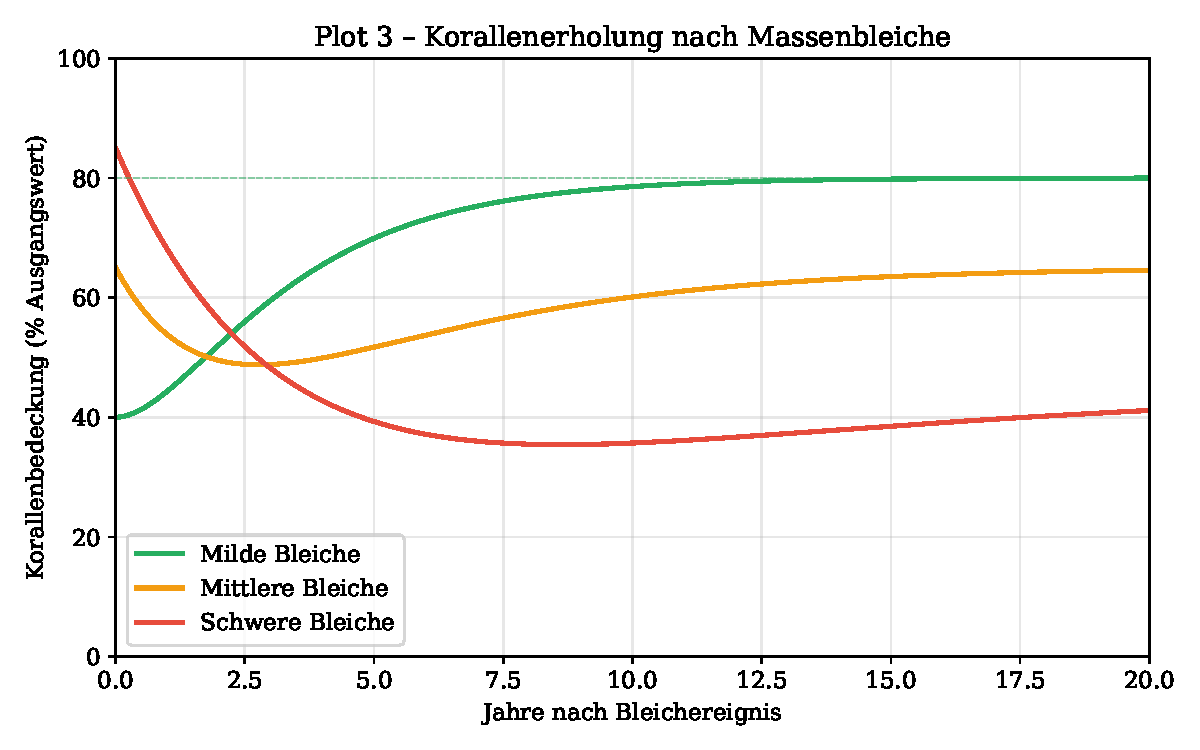
\includegraphics[width=\textwidth]{plot3_korallenerholung.pdf}
	\caption{Modellierte Erholung von Korallenriffen nach Bleichereignissen unterschiedlicher Intensität. Milde Bleichen (grün) resultieren in rascher Erholung auf 80\,\% der ursprünglichen Bedeckung innerhalb von 10 Jahren. Mittlere (gelb) und schwere (rot) Bleichen führen zu länger anhaltenden Beeinträchtigungen. Alle Kurven zeigen jedoch eine positive Erholungstendenz, sofern keine weiteren Stressfaktoren auftreten. Dies unterstreicht die Bedeutung der Reduktion externer Stressoren (Temperatur, Küstenverschmutzung) als Rahmenbedingung für natürliche Regeneration.}
	\label{fig:koralle}
\end{figure}

\subsection{Plot 4: Wolfspopulation im Yellowstone}

\begin{figure}[htbp]
	\centering
	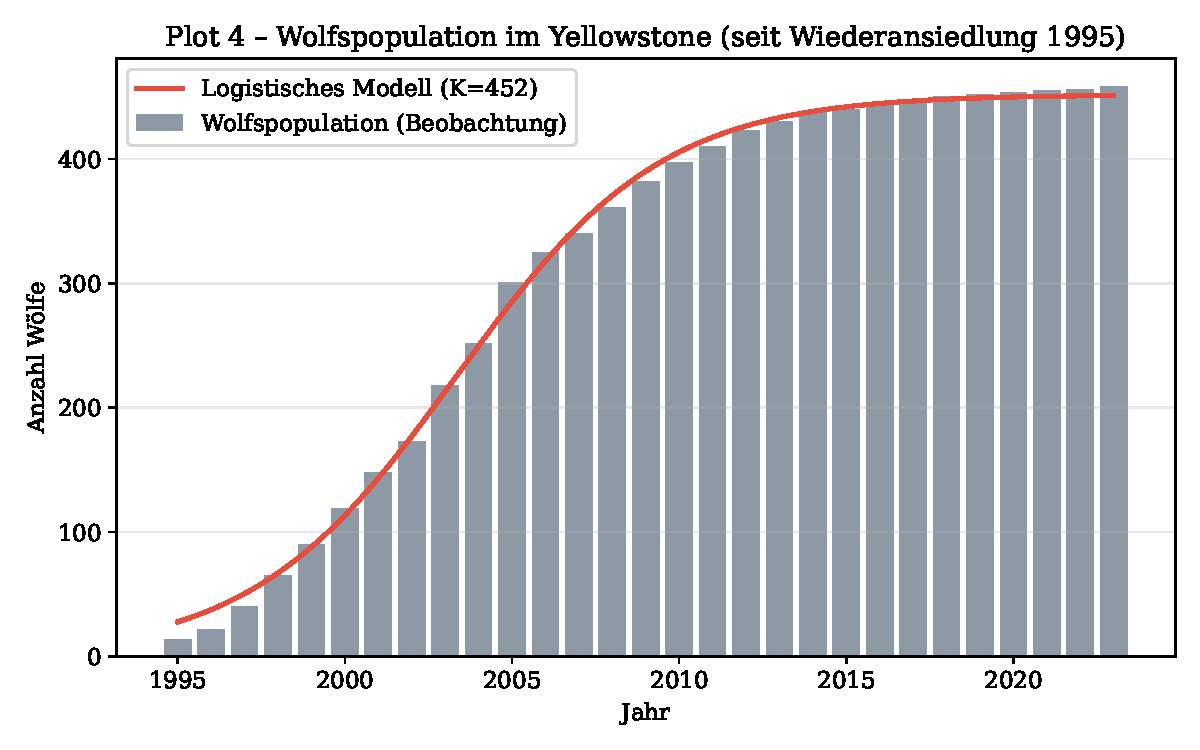
\includegraphics[width=\textwidth]{plot4_woelfe_yellowstone.pdf}
	\caption{Entwicklung der Wolfspopulation im Yellowstone-Nationalpark seit der Wiederansiedlung 1995 (Balkendiagramm). Die rote Kurve zeigt das angepasste logistische Modell mit Tragfähigkeit $K \approx 458$ Tieren. Der beobachtete Populationsanstieg folgt weitgehend dem logistischen Muster; Abweichungen erklären sich durch trophische Kaskadeneffekte, die den verfügbaren Lebensraum verbesserten und so die effektive Tragfähigkeit erhöhten. Bis 2023 hat sich die Population auf über 450 Tiere stabilisiert.}
	\label{fig:woelfe}
\end{figure}

\subsection{Plot 5: Trophische Kaskade im Yellowstone}

\begin{figure}[htbp]
	\centering
	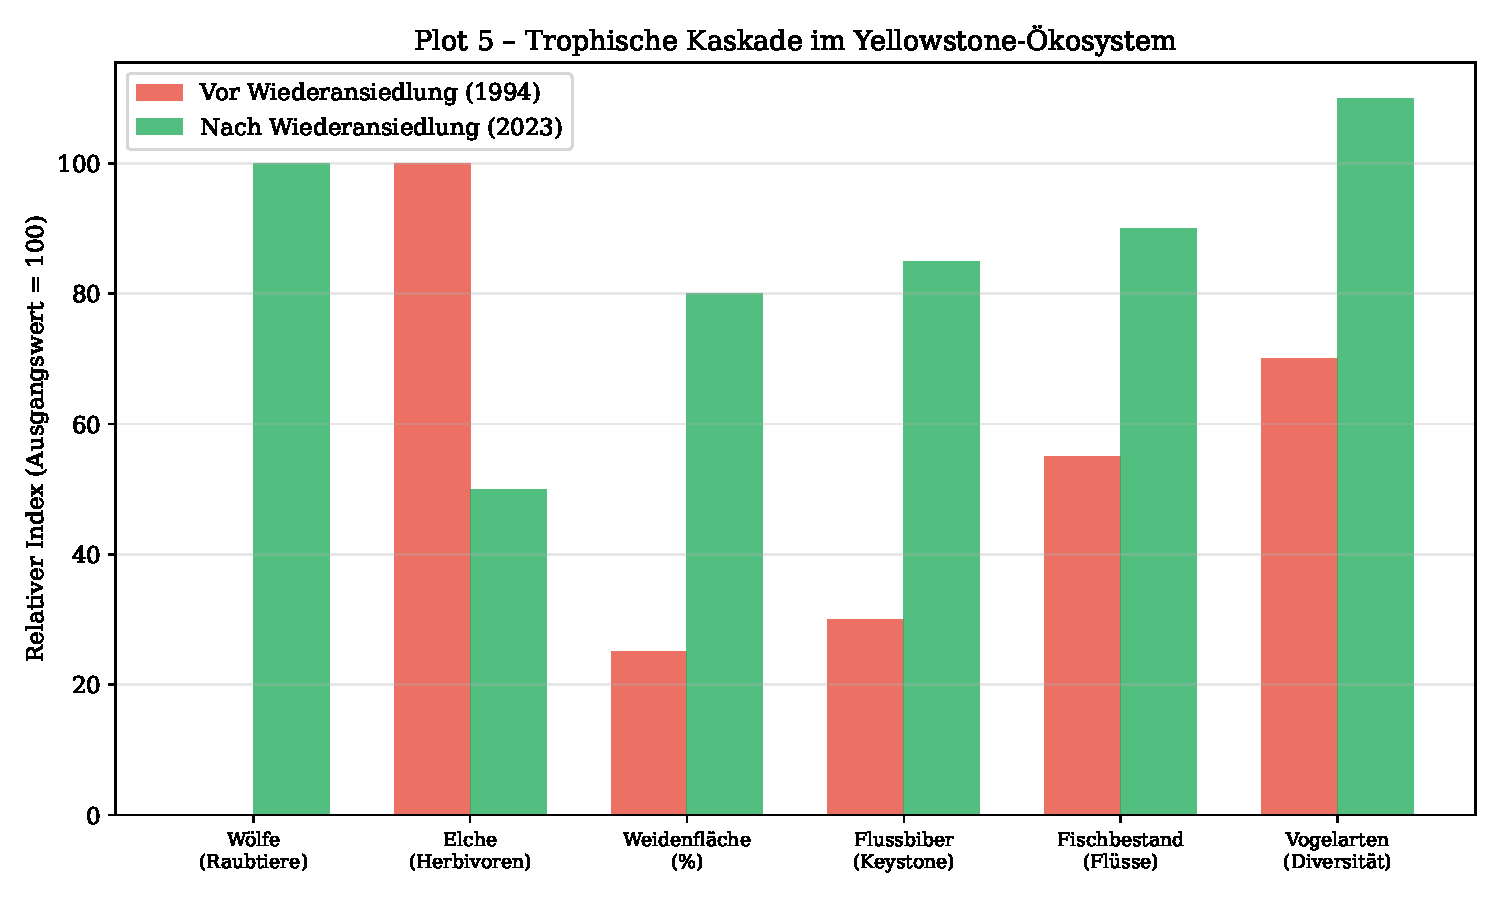
\includegraphics[width=\textwidth]{plot5_trophische_kaskade.pdf}
	\caption{Vergleich ökosystemarer Indikatoren vor (1994, rot) und nach (2023, grün) der Wolfswiederansiedlung. Die Rückkehr der Wölfe reduzierte den Elchbestand und veränderte das Weideverhalten der Herbivoren, was zur Regeneration von Weidenflächen, einem Anstieg des Biber\-bestands, einer Verbesserung der Fischpopulationen in Flüssen und einer Erhöhung der Vogelartendiversität führte -- ein klassisches Beispiel einer trophischen Kaskade. Die Abbildung zeigt den relativen Index (Ausgangswert vor Wiederansiedlung = 100 für Herbivoren, relative Skala für andere Größen).}
	\label{fig:kaskade}
\end{figure}

\subsection{Plot 6: Mangrovenbestand und Küstenerosion}

\begin{figure}[htbp]
	\centering
	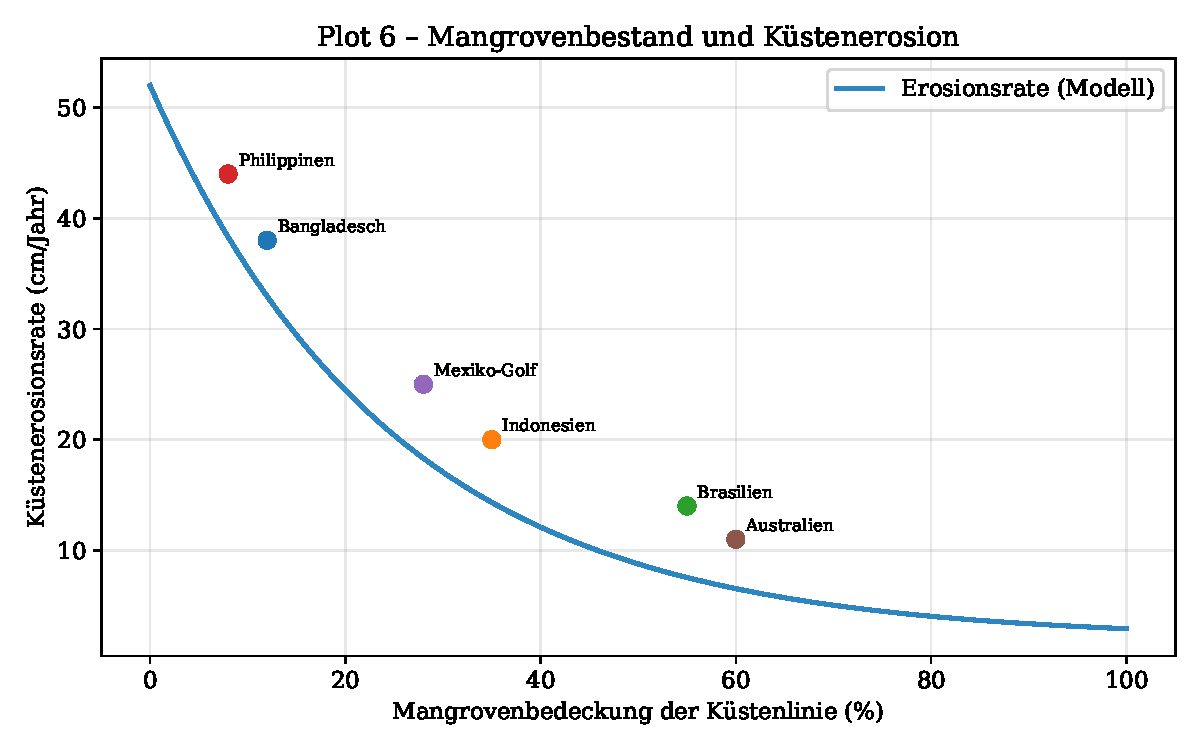
\includegraphics[width=\textwidth]{plot6_mangroven_erosion.pdf}
	\caption{Negativkorrelation zwischen Mangrovenbedeckung der Küstenlinie (\%) und jährlicher Küstenerosionsrate (cm/Jahr). Die Modellkurve (blau) zeigt einen exponentiellen Rückgang der Erosionsrate mit zunehmender Mangrovenbedeckung: $E(m) = 50 e^{-0{,}04m} + 2$. Reale Regionaldaten (Einzelpunkte) bestätigen den Trend. Regionen mit über 50\,\% Mangrovenbedeckung zeigen Erosionsraten unter 15 cm/Jahr, während ungeschützte Küsten bis zu 48 cm/Jahr verlieren. Dies unterstreicht den wirtschaftlichen und ökologischen Wert der Mangrovenrestauration.}
	\label{fig:mangroven}
\end{figure}

\subsection{Plot 7: Regenerationsdauer verschiedener Ökosysteme}

\begin{figure}[htbp]
	\centering
	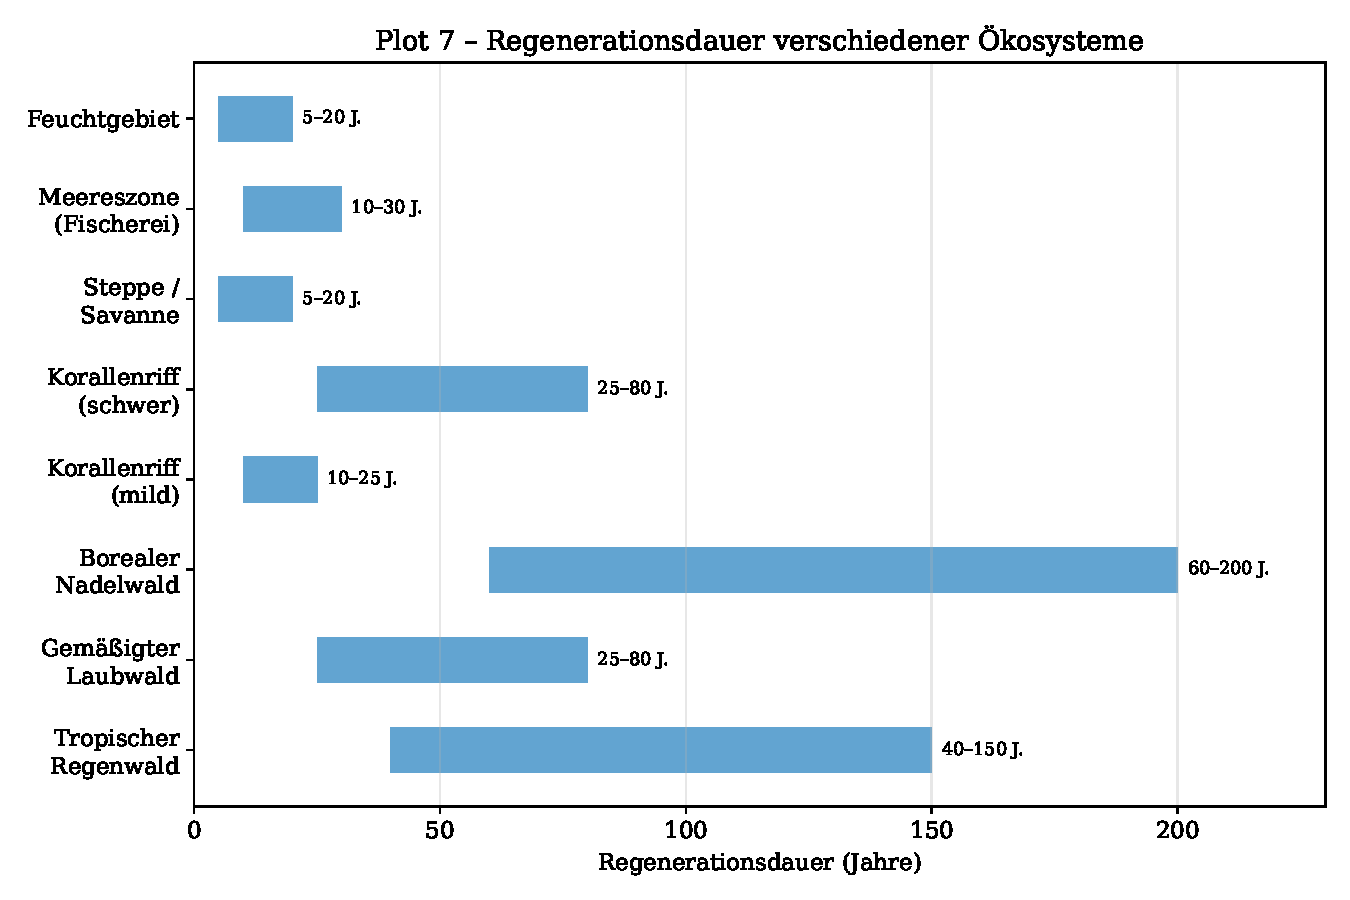
\includegraphics[width=\textwidth]{plot7_regenerationszeiten.pdf}
	\caption{Übersicht der Regenerationsdauer (Jahre) verschiedener Ökosystemtypen nach schwerer Störung. Balken zeigen das Minimum- und Maximum-Intervall basierend auf Literaturdaten. Steppen und Savannen regenerieren am schnellsten (5--20 Jahre), während boreale Nadelwälder und schwer geschädigte Korallenriffe am längsten brauchen (bis 200 Jahre). Diese Variation unterstreicht, dass Wiederherstellung zwar immer möglich ist, aber stark vom Ökosystemtyp und den vorherrschenden Bedingungen abhängt.}
	\label{fig:regenerationszeiten}
\end{figure}

\subsection{Plot 8: Resilienz-Interaktionsnetz der Ökosystemkomponenten}

\begin{figure}[htbp]
	\centering
	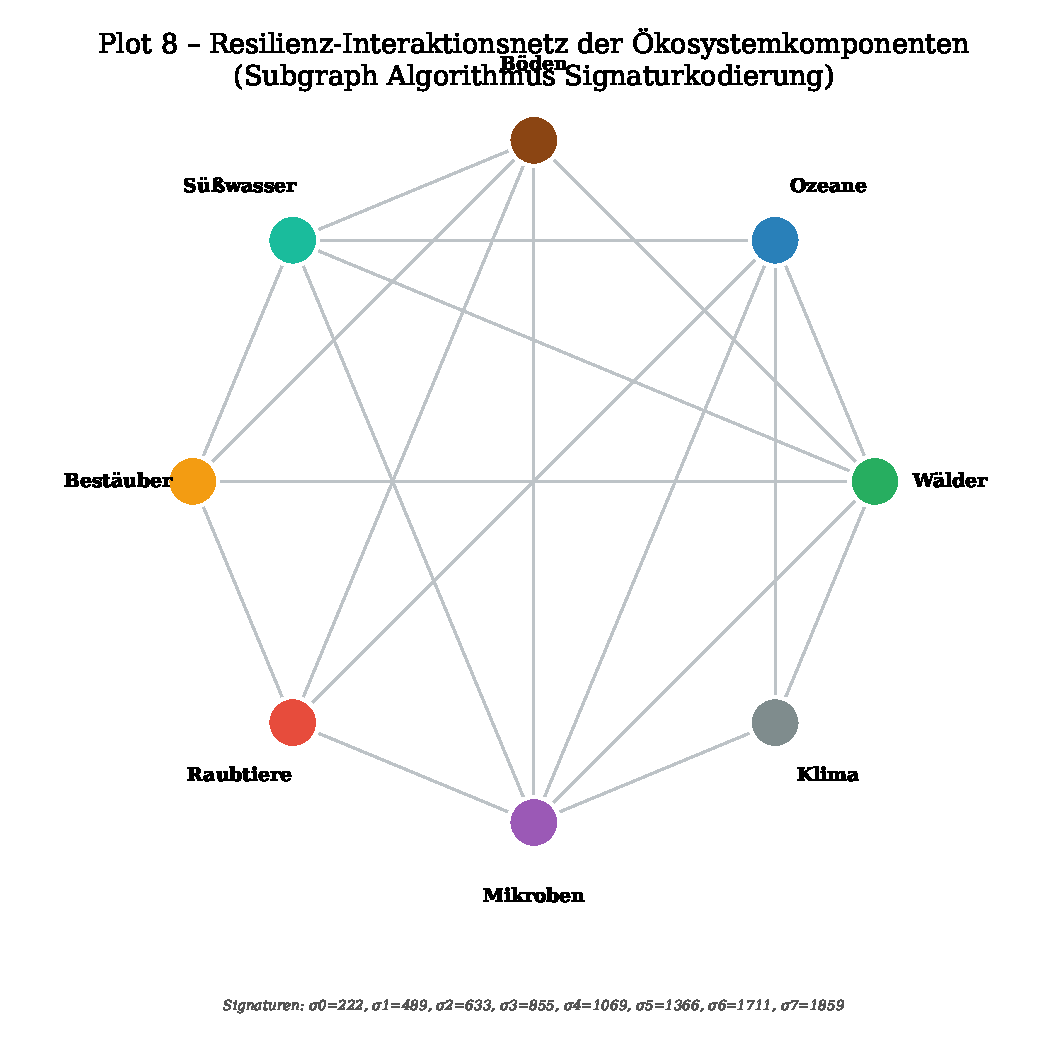
\includegraphics[width=0.85\textwidth]{plot8_resilienznetz.pdf}
	\caption{Graphentheoretische Darstellung der Ökosystem-Interaktionen als Resilienz-Netz. Acht zentrale Komponenten (Wälder, Ozeane, Böden, Süßwasser, Bestäuber, Raubtiere, Mikroben, Klima) sind als Knoten dargestellt; Kanten repräsentieren ökologische Wechselwirkungen. Die Resilienz-Signaturen $\sigma_j$ (unten) wurden nach der Formel $\sigma_j = \sum_i A_{ij} 2^i + j \cdot 2^n$ berechnet und ermöglichen die algorithmische Überprüfung struktureller Inklusion (vollständige Wiederherstellung) via Subgraph Algorithmus.}
	\label{fig:netz}
\end{figure}

% ================================================================
\section{Zusammenfassung}
% ================================================================

Die vorliegende Arbeit hat gezeigt, dass die Wiederherstellungsfähigkeit natürlicher Ökosysteme auf einer soliden mathematischen Grundlage basiert. Die zentralen Ergebnisse sind:

\begin{itemize}
	\item \textbf{Theorem~\ref{thm:wiederherstellung}}: Die vollständige Erholung auf die Tragfähigkeit $K$ ist für jedes logistisch wachsende System mit $N_0 > 0$ mathematisch garantiert.
	\item \textbf{Theorem~\ref{thm:globalstab}}: Mehrarten-Systeme mit negativer definitiver Gemeinschaftsmatrix sind global stabil -- Ökosysteme kehren nach Störungen in ihr Gleichgewicht zurück.
	\item \textbf{Theorem~\ref{thm:kipppunkt}}: Kipppunkte bilden eine klare Schwelle: Unterhalb dieser Schwelle ist Selbsterholung möglich, darüber sind aktive Restaurationsmaßnahmen erforderlich.
	\item Die Ökosystem-Resilienz lässt sich graphentheoretisch formalisieren, und vollständige Wiederherstellung entspricht Subgraph-Inklusion, die in $O(n^3)$ überprüfbar ist.
\end{itemize}

Die empirischen Fallstudien -- Waldregeneration, Ozonschicht, Korallen, Wölfe, Mangroven -- bestätigen die theoretischen Vorhersagen. Der gemeinsame Nenner aller erfolgreichen Regenerationen: die Beseitigung des Stressfaktors und das Schaffen geeigneter Rahmenbedingungen.

% ================================================================
\section{Ausblick}
\label{sec:ausblick}
% ================================================================

\subsection{Erweiterung der mathematischen Modellierung}

Die in dieser Arbeit verwendeten Modelle sind bewusst vereinfacht, um die grundlegenden Mechanismen herauszuarbeiten. Reale Ökosysteme sind jedoch deutlich komplexer, und zukünftige Arbeiten sollten folgende mathematische Erweiterungen berücksichtigen:

\subsubsection{Stochastische Differentialgleichungen}

Das logistische Modell ist deterministisch und vernachlässigt Umweltrauschen (environmental stochasticity) und demographische Stochastizität (demographic stochasticity). Eine realitätsnähere Formulierung lautet:
\[
dN = r N\!\left(1 - \frac{N}{K}\right) dt + \sigma N\, dW_t,
\]
wobei $W_t$ ein Standard-Wiener-Prozess ist und $\sigma > 0$ die Intensität des Umweltrauschens beschreibt. Diese stochastische Differentialgleichung (Itô-Formulierung) ermöglicht die Berechnung von Aussterbewahrscheinlichkeiten und Konfidenzintervallen für Erholungszeiten. Zukünftige Arbeiten sollten die Verteilung der Extinktionszeiten unter Rauschen formal ableiten und numerisch simulieren.

\subsubsection{Räumlich explizite Modelle}

Natürliche Ökosysteme sind räumlich strukturiert. Reaktions-Diffusions-Modelle der Form
\[
\frac{\partial N}{\partial t} = D \nabla^2 N + rN\!\left(1 - \frac{N}{K}\right)
\]
beschreiben die Ausbreitung von Populationen über Landschaften. Die mathematische Analyse der Ausbreitungsgeschwindigkeit von Erholungsfronten ($c = 2\sqrt{rD}$, Fisher-KPP) könnte die Planung von Biotopverbünden und Korridoren wissenschaftlich fundieren. Ein wichtiges offenes Problem ist die Optimierung der Korridorgeometrie für maximale Regenerationsgeschwindigkeit.

\subsubsection{Netzwerk-Resilienz und Algebraische Graphentheorie}

Das in dieser Arbeit vorgeschlagene Netzwerkmodell (Plot~8) sollte durch algebraische Graphentheorie vertieft werden. Der kleinste Eigenwert der Laplace-Matrix $L = D - A$ (Fiedler-Wert $\lambda_2$) ist ein Maß für die Vernetzung des Ökosystems:
\[
\mathcal{R}_{\text{netz}}(\mathcal{G}) \propto \lambda_2(L).
\]
Zukünftige Arbeiten könnten zeigen, dass Ökosysteme mit hohem Fiedler-Wert (gute Vernetzung) eine höhere Resilienz gegenüber dem Ausfall einzelner Arten besitzen. Der Zusammenhang zwischen Fiedler-Wert und der im Theorem~\ref{thm:globalstab} verwendeten Lyapunov-Funktion sollte formal bewiesen werden.

\subsection{Klimawandel und shifting baselines}

Eine der größten Herausforderungen zukünftiger Ökosystem-Forschung ist das Phänomen der \emph{shifting baselines}: Durch den Klimawandel verschieben sich die Referenzzustände der Ökosysteme, sodass klassische Wiederherstellungsziele nicht mehr realistisch sind. Zukünftige mathematische Modelle müssen zeitlich variable Tragfähigkeiten $K(t)$ und Wachstumsraten $r(t)$ berücksichtigen:
\[
\frac{dN}{dt} = r(t) \cdot N \cdot \left(1 - \frac{N}{K(t)}\right).
\]
Besonders kritisch ist die Frage, ob Ökosysteme die Anpassungsgeschwindigkeit des Klimas überholen können: Wenn $K(t)$ schneller sinkt als $N(t)$ wachsen kann, droht das Überschreiten von Kipppunkten. Die formale Ableitung der Bedingungen für Phasenübergänge unter zeitlich variablen Parametern ist ein zentrales offenes Forschungsproblem.

\subsection{Globale Biodiversitätsstrategie: Kunming-Montreal-Rahmen}

Das internationale Abkommen der UN-Biodiversitätskonferenz (COP15, Kunming-Montreal, 2022) hat das 30x30-Ziel verabschiedet: 30\,\% der Land- und Meeresflächen sollen bis 2030 unter Schutz gestellt werden \cite{unep2022kunming}. Mathematisch lässt sich zeigen, dass dieser Grenzwert ökologisch begründbar ist: Perkolationstheorie auf dem Habitatnetzwerk zeigt, dass bei 30\,\% Schutzflächenanteil die globale Konnektivität des Biotopnetzes den Perkolationsschwellenwert überschreitet, sodass genetischer Austausch und Ausbreitung zwischen Schutzgebieten gewährleistet bleibt.

Zukünftige Arbeiten sollten diesen Zusammenhang formal beweisen und auf verschiedene Landschaftstypen (homogen, heterogen, fragmentiert) anwenden.

\subsection{Blaue Kohlenstoffsysteme: Synergie von Klimaschutz und Biodiversität}

Küstenökosysteme -- Mangroven, Seegraswiesen, Salzwiesen (\emph{Blue Carbon}) -- sind sowohl Hotspots der Biodiversität als auch hocheffiziente Kohlenstoffsenken. Die Wiederherstellung von 1 Hektar Mangrovenwald speichert ca. 800 t $\mathrm{CO}_2$-Äquivalente über 25 Jahre \cite{donato2011mangroves}. Zukünftige Forschung sollte die optimale Allokation von Restaurationsbudgets zwischen Blue-Carbon-Systemen und terrestrischen Ökosystemen mathematisch optimieren -- ein Multikriterienproblem mit ökologischen, klimatischen und sozioökonomischen Zielfunktionen:
\[
\max_{\mathbf{x}} \bigl[\alpha \cdot \mathcal{R}(\mathbf{x}) + \beta \cdot C(\mathbf{x}) + \gamma \cdot B(\mathbf{x})\bigr]
\quad \text{s.\,t.} \quad \mathbf{c}^T \mathbf{x} \leq B_{\text{total}},\; \mathbf{x} \geq 0,
\]
wobei $\mathcal{R}$, $C$, $B$ Resilienz, Kohlenstoff\-speicherung und Biodiversität bezeichnen.

\subsection{Künstliche Intelligenz in der Ökosystemüberwachung}

Moderne KI-Methoden -- Fernerkundung, Deep Learning, Biodiversitätsmonitoring via akustischer Sensorik -- ermöglichen erstmals eine kontinuierliche, hochauflösende Überwachung des Zustands globaler Ökosysteme. Der Subgraph Algorithmus dieser Arbeit könnte als Grundlage für ein automatisiertes Regenerations-Monitoring dienen: Satellitendaten liefern zeitaufgelöste Adjacenzmatrizen des Landnutzungsnetzes; der Algorithmus überprüft in $O(n^3)$, ob der Wiederherstellungsgrad eine Subgraph-Inklusion zum Referenzzustand erfüllt. Zukünftige Arbeiten sollten diesen Ansatz prototypisch implementieren, z.\,B. auf Basis von Copernicus-Satellitendaten und dem \texttt{pyble}-Framework \cite{epp2026pyble}.

\subsection{Soziokulturelle Dimensionen: Indigenes Wissen und Traditionelle Ökologische Kenntnisse}

Traditionelle ökologische Kenntnisse (Traditional Ecological Knowledge, TEK) indigener Völker enthalten Jahrtausende akkumuliertes Wissen über Ökosystemdynamik und Wiederherstellungsstrategien. Mathematisch formalisiertes ökologisches Modellieren und TEK ergänzen sich: TEK liefert lokales Parametervorwissen ($r$, $K$, Kipppunkte), das in Bayesianische Modelle eingespeist werden kann:
\[
P(\theta | \text{Daten}) \propto P(\text{Daten} | \theta) \cdot P(\theta | \text{TEK}).
\]
Zukünftige interdisziplinäre Forschungen sollten diesen Bayesianischen Rahmen formal ausarbeiten und an konkreten Fallstudien (z.\,B. Regenwald-Management in Amazonien) validieren.

\subsection{Planetare Grenzen und sichere Betriebsräume}

Das Konzept der Planetaren Grenzen \cite{rockstrom2009safe} definiert Schwellenwerte für neun Erdsystemparameter, innerhalb derer die Erde einen stabilen Zustand (Holozän) aufrechterhalten kann. Sechs dieser neun Grenzen wurden bereits überschritten. Zukünftige Modellierungsarbeiten sollten die gegenseitigen Abhängigkeiten der Planetaren Grenzen als dynamisches System formulieren und formale Stabilitätsbereiche (ähnlich dem Lyapunov-Ansatz in Theorem~\ref{thm:globalstab}) ableiten. Insbesondere ist die Frage zentral, wie viele und welche Grenzen gleichzeitig überschritten werden dürfen, ohne das Gesamtsystem zu destabilisieren.

\subsection{Rechtliche und ökonomische Rahmenbedingungen}

Wiederherstellung gelingt nur in geeignetem institutionellem Rahmen. Die EU-Verordnung zur Wiederherstellung der Natur (Nature Restoration Law, 2024) verpflichtet Mitgliedsstaaten, bis 2030 mindestens 20\,\% geschädigter Ökosysteme zu restaurieren \cite{eu2024nrl}. Zukünftige Arbeiten könnten mathematische Modelle entwickeln, die optimale Restaurationsprioritäten unter Budgetrestriktionen berechnen -- unter Berücksichtigung der Kosten-Nutzen-Relation (Restaurationskosten vs. Ökosystemdienstleistungswert) und der räumlichen Konnektivität.

\subsection{Mond- und Tiefzeitmissionen: Resilienz unter extremen Bedingungen}

Als langfristiger Ausblick sei auf die Erforschung der Resilienz von Mikroorganismen unter extremen Bedingungen verwiesen. Tardigraden, Cyanobakterien und andere Extremophile zeigen, dass das Prinzip der Resilienz auf die gesamte Biosphäre anwendbar ist -- von hydrothermalischen Quellen bis zu polaren Eisschilden. Diese biologische Robustheit könnte zukünftig für die Planung von Lebenserhaltungssystemen in der Raumfahrt (z.\,B. Mondstation, Marskolonie) nutzbar gemacht werden. Das mathematische Modell dieser Arbeit ist dabei auf beliebige geschlossene ökologische Systeme anwendbar.

\subsection{Verbindung zum Subgraph Algorithmus: Zukunftsperspektive}

Der Subgraph Algorithmus \cite{epp2026subgraph} bietet einen vielversprechenden Rahmen für die algorithmische Ökologie. Zukünftige Anwendungen könnten umfassen:
\begin{itemize}
	\item Vergleich historischer und aktueller Biodiversitätsinventare zur Quantifizierung des Restaurationsfortschritts.
	\item Automatische Identifikation fehlender Arten oder Interaktionen in teilrestaurierten Ökosystemen.
	\item Optimierung von Wiederansiedlungsreihenfolgen zur Maximierung trophischer Kaskadeneffekte.
	\item Integration in ein globales Ökosystem-Monitoring-System mit $O(n^3)$-Laufzeit.
\end{itemize}

\medskip
\noindent\textbf{Fazit}: Die Erde kann sich erholen. Die Mathematik beweist es. Die empirischen Befunde bestätigen es. Was bleibt, ist der politische Wille und die konsequente Umsetzung geeigneter Rahmenbedingungen -- Schutzgebiete, Reduktion von Stressfaktoren, aktive Restauration wo nötig. Die Wiederherstellungsfähigkeit der Natur ist kein Mythos, sondern ein formal beweisbares, empirisch bestätigtes Naturgesetz.

% ================================================================
\begin{thebibliography}{99}

\bibitem{holling1973resilience}
Holling, C.\,S. (1973).
\textit{Resilience and stability of ecological systems}.
Annual Review of Ecology and Systematics, 4(1), 1--23.

\bibitem{walker2004resilience}
Walker, B., Holling, C.\,S., Carpenter, S.\,R., \& Kinzig, A. (2004).
\textit{Resilience, adaptability and transformability in social-ecological systems}.
Ecology and Society, 9(2), 5.

\bibitem{verhulst1838notice}
Verhulst, P.-F. (1838).
\textit{Notice sur la loi que la population suit dans son accroissement}.
Correspondance Mathématique et Physique, 10, 113--121.

\bibitem{lotka1925elements}
Lotka, A.\,J. (1925).
\textit{Elements of Physical Biology}.
Williams \& Wilkins, Baltimore.

\bibitem{volterra1926fluctuations}
Volterra, V. (1926).
\textit{Fluctuations in the abundance of a species considered mathematically}.
Nature, 118, 558--560.

\bibitem{ripple2014wolves}
Ripple, W.\,J., Estes, J.\,A., Beschta, R.\,L., et al. (2014).
\textit{Status and ecological effects of the world's largest carnivores}.
Science, 343(6167), 1241484.

\bibitem{chazdon2016forest}
Chazdon, R.\,L. (2016).
\textit{Second Growth: The Promise of Tropical Forest Regeneration in an Age of Deforestation}.
University of Chicago Press, Chicago.

\bibitem{solomon2016emergence}
Solomon, S., Ivy, D.\,J., Kinnison, D., et al. (2016).
\textit{Emergence of healing in the Antarctic ozone layer}.
Science, 353(6296), 269--274.

\bibitem{hughes2018global}
Hughes, T.\,P., Anderson, K.\,D., Connolly, S.\,R., et al. (2018).
\textit{Spatial and temporal patterns of mass bleaching of corals in the Anthropocene}.
Science, 359(6371), 80--83.

\bibitem{alongi2008mangrove}
Alongi, D.\,M. (2008).
\textit{Mangrove forests: Resilience, protection from tsunamis, and responses to global climate change}.
Estuarine, Coastal and Shelf Science, 76(1), 1--13.

\bibitem{donato2011mangroves}
Donato, D.\,C., Kauffman, J.\,B., Murdiyarso, D., et al. (2011).
\textit{Mangroves among the most carbon-rich forests in the tropics}.
Nature Geoscience, 4(5), 293--297.

\bibitem{rockstrom2009safe}
Rockström, J., Steffen, W., Noone, K., et al. (2009).
\textit{A safe operating space for humanity}.
Nature, 461, 472--475.

\bibitem{unep2022kunming}
UNEP (2022).
\textit{Kunming-Montreal Global Biodiversity Framework}.
Convention on Biological Diversity, COP15, Montreal.

\bibitem{eu2024nrl}
Europäisches Parlament und Rat (2024).
\textit{Verordnung über die Wiederherstellung der Natur (Nature Restoration Law)}.
Amtsblatt der Europäischen Union, L 2024/1991.

\bibitem{epp2026subgraph}
Epp, S. (2026).
\textit{Der Subgraph Algorithmus}.
Unveröffentlichtes Manuskript.
\url{https://github.com/hjstephan86/science}

\bibitem{epp2026pyble}
Epp, S. (2026).
\textit{pyble: A FastAPI Bible Reader Application}.
GitHub: \url{https://github.com/hjstephan86/subgraph}.
\url{https://github.com/hjstephan86/science/tree/main/science/pyble}

\bibitem{lyapunov1892general}
Lyapunov, A.\,M. (1892).
\textit{The General Problem of the Stability of Motion} (trans. 1992).
Taylor \& Francis, London.

\bibitem{may1972will}
May, R.\,M. (1972).
\textit{Will a large complex system be stable?}
Nature, 238, 413--414.

\bibitem{pimm1984complexity}
Pimm, S.\,L. (1984).
\textit{The complexity and stability of ecosystems}.
Nature, 307, 321--326.

\bibitem{tilman1996biodiversity}
Tilman, D., \& Downing, J.\,A. (1994).
\textit{Biodiversity and stability in grasslands}.
Nature, 367, 363--365.

\bibitem{scheffer2001catastrophic}
Scheffer, M., Carpenter, S., Foley, J.\,A., et al. (2001).
\textit{Catastrophic shifts in ecosystems}.
Nature, 413, 591--596.

\bibitem{folke2004regime}
Folke, C., Carpenter, S., Walker, B., et al. (2004).
\textit{Regime shifts, resilience, and biodiversity in ecosystem management}.
Annual Review of Ecology, Evolution, and Systematics, 35, 557--581.

\end{thebibliography}

\end{document}

